\section{Auswertung}
\label{sec:Auswertung}
Die Lamorfrequenz der Protonen wird als \SI{21.71134}{\mega\hertz} bestimmt und die ideale Phase ergibt sich als \SI{115}{\degree}.
Eine maximale Amplitude der FID wurde bei $t =  \SI{2.76}{\micro\second}$ gemessen und bei $t = \SI{5.14}{\micro\second}$ verschwindet besagte Amplitude.
Diese Zeiten geben daher die Pulslängen für einen \SI{90}{\degree} und einen \SI{180}{\degree} Impuls.
Die Temperatur der Spule zum Zeitpunkt der Messung wird als \SI{21.1}{\celsius} bestimmt.

\subsection{Bestimmung der $T_1$-Relaxationszeit}
In Abbildung \ref{fig:df1} sind die Messwerte für die $T_1$ Messung dargestellt, außerdem wurde an die Daten eine Funktion der Form
\begin{equation}
    A\left(\tau\right) = A_0 \left(1-2\exp\left( - \frac{\tau}{T_1}\right)\right)
\end{equation}
gefittet.
Durch das annähern der Funktion ergeben sich folgende Parameter: 
\begin{align*}
    A_0 &= \SI{2.1912 +- 0.0226}{\volt}\\
    T_1 &= \SI{2.784 +- 0.04}{\second}
\end{align*}
Dabei entspricht der Parameter $T_1$ der hier gesuchten Spin-Gitter-Relaxationszeit
\begin{figure}[ht]
    \center
    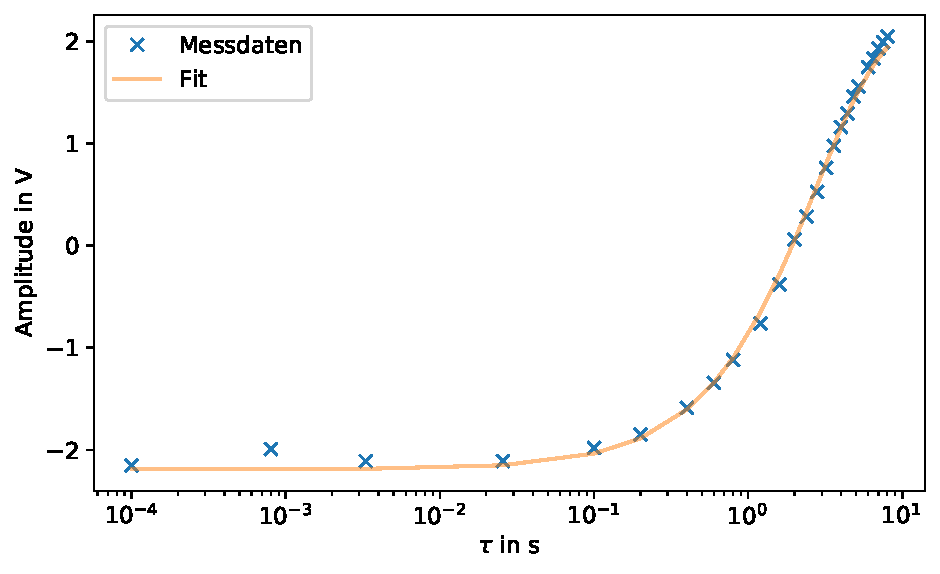
\includegraphics[scale = 0.75]{plots/df1.pdf}
    \caption{Amplitude der FID aufgetragen gegen die Pulslänge $\tau$. Mithilfe des Fits kann die Spin-Gitter-Relaxationszeit bestimmt werden. DIe Pulslängen werden in logarithmischer Form aufgetragen.}
    \label{fig:df1}
\end{figure}
\newpage
\subsection{Bestimmung der $T_2$-Relaxationszeit}
Wenn nun der $\alpha_{90°}$ Puls und der $\alpha_{180°}$ Puls in Phase sind (ausgeschaltetes 'MG') lässt sich die $T_2$ Relaxationszeit nicht bestimmen wie in Abbildung \ref{fig:df54} gezeigt.
Bei eingeschaltetem 'MG' lässt sich anhand der Peaks in der Messung die Relaxationszeit bestimmen, siehe Abbildung \ref{fig:df52}.
\begin{figure}[H]
    \center
    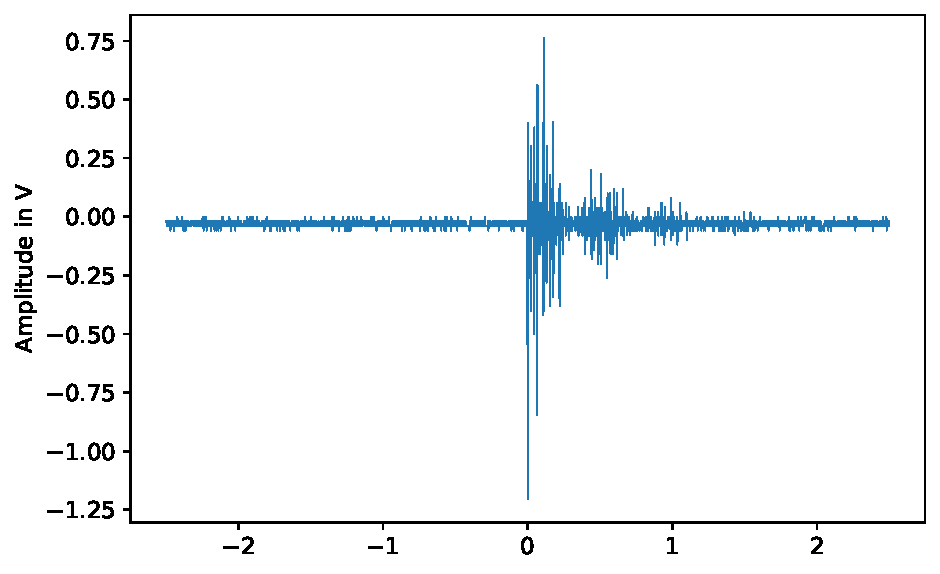
\includegraphics[scale = 0.75]{plots/df54.pdf}
    \caption{Amplitude aufgetragen gegen die Pulsabstände. In diesem Fall ist das 'MG' ausgeschaltet und die beiden Pulse daher nicht in Phase. Die Pulse sind erkennbar, allerdings ist kein Rückschluss auf die Relaxationszeit möglich.} 
    \label{fig:df54}
\end{figure}
Nach der Bestimmung der Peaks mit einer 'scipy' Methode \cite{2020SciPy-NMeth} wird eine Funktion der Form
\begin{equation*}
    A\left(\tau\right) = A_0 \left(1 + 2\exp\left( - \frac{\tau}{T_2}\right)\right)
\end{equation*}
an die Peaks gefittet um $T_2$ zu bestimmen.
\begin{figure}[ht]
    \center
    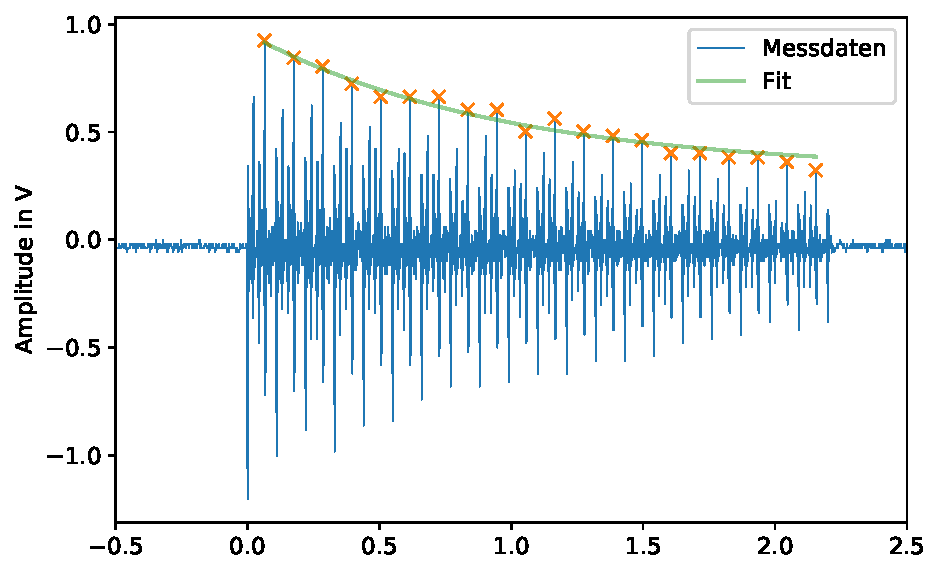
\includegraphics[scale = 0.75]{plots/df52.pdf}
    \caption{Die Amplitude für den Fall dass die Pulse in Phase sind. An die Peaks der Messung wird ein Fit genähert zur Bestimmung der Relaxationszeit. Das Rauschen an beiden Seiten wurde der Übersicht halber zum großteil weggeschnitten.}
    \label{fig:df52}
\end{figure}
Mit dem nähern der Funktion ergeben sich folgende Parameter:
\begin{align*}
    A_0 &= \SI{0.319 +- 0.009}{\volt}\\
    T_2 &= \SI{0.95 +- 0.08}{\second}
\end{align*}
In diesem Fall entspricht $T_2$ der gesuchten Spin-Spin-Relaxationszeit.
\newpage
\subsection{Bestimmung der Diffusionszeit $T_D$}
Zunächst wird eine Funktion der Amplitude $f(A) = ln(A(\tau)) - \frac{2\tau}{T_2}$ gegen die Relaxationszeit hoch drei $\tau^3$ aufgetragen. 
Diese Größen sollten proportional zueinander sein, jedoch ist dieser Zusammenhang nur für kleine $\tau$ zu erkennen.
Um Aussagekräftigere Ergebnisse zu erhalten wird die Amplitude direkt gegen die Relaxationszeit in $10^3 \si{\second}$ aufgetragen und eine Funktion der Form
\begin{equation*}
    A\left(\tau\right) = A_0 \exp\left(- \frac{2\tau}{T_2}\right) \exp\left(-\frac{\tau^3}{T_D}\right)
\end{equation*}
an die Daten gefittet, siehe Abbildung \ref{fig:df2_2}.
\begin{figure}[ht]
    \center
    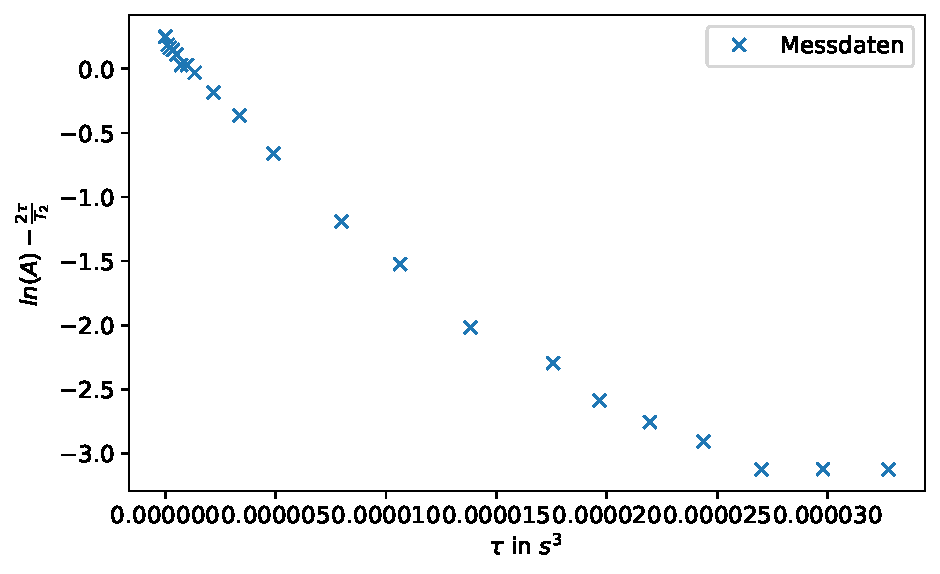
\includegraphics[scale = 0.75]{plots/df2.pdf}
    \caption{Der entsprechende Logarithmus der Amplitude wird gegen die Relaxationszeit hoch drei aufgetragen. Die Abhängigkeit der Größen lässt eine lineare Funktion erwarten, allerdings ist diese Linearität nur für kleine $\tau$ zu erkennen.}
    \label{fig:df2}
\end{figure}
\begin{figure}[ht]
    \center
    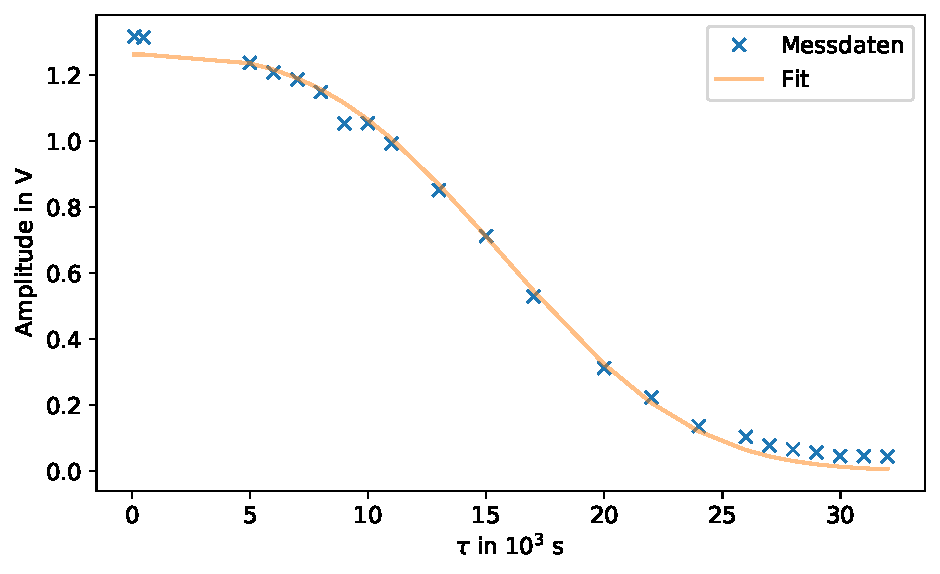
\includegraphics[scale = 0.75]{plots/df2_2.pdf}
    \caption{Die Amplitude aufgetragen gegen die Pulsdauer. An die Messwerte wurde die Funktion zur bestimmung der Diffusionszeit genähert.}
    \label{fig:df2_2}
\end{figure}
Mit dem Fit ergeben sich folgende Parameter:
\begin{align*}
    A_0 &= \SI{1.2897 +- 0.0127}{\volt}\\
    T_D &= \SI{5.876 +- 0.207}{\second}
\end{align*}
Dabei ist $T_D$ die gesuchte Diffusionszeit.

\subsection{Berechnung des Feldgradienten $G$}
In Abbildung \ref{fig:fourier} ist die Fouriertransformierte des Signals, dessen Real und Imaginärteil in Abbildung \ref{fig:df58_59} zu sehen ist,gezeigt.
Die Fouriertransformierte bildet annähernd einen Halbkreis, dessen Durchmesser als $k = \SI{8.450 +- 0.10}{\kilo\hertz}$ abgelesen wird.
Zusammen mit dem gyromagnetischen Verhältnis von Protonen  $\gamma = \SI[per-mode=fraction]{2.67E08}{\per\tesla\per\second}$ und der Dicke der Probe $d = \SI{0.0044}{\metre}$ lässt sich daraus der Feldgradient berechnen.
\begin{equation}
    G = \frac{2\pi k}{\gamma d} = \SI{0.0451+-0.0005}{\tesla\per\metre}
\end{equation}
\begin{figure}[ht]
    \center
    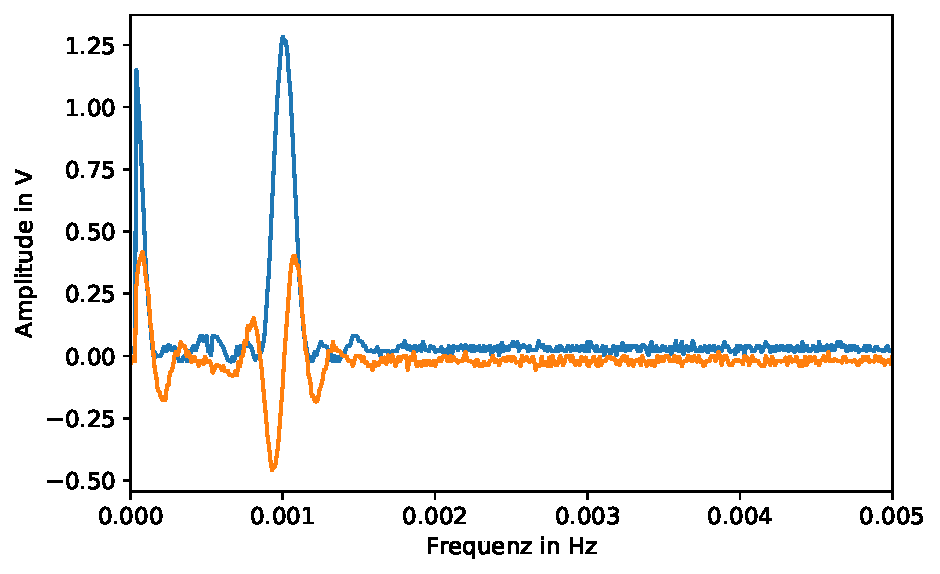
\includegraphics[scale = 0.75]{plots/df58_59.pdf}
    \caption{Real und Imaginärteil des Spin-Echos zur Bestimmung der Diffusionskonstanten}
    \label{fig:df58_59}
\end{figure}
\begin{figure}[ht]
    \center
    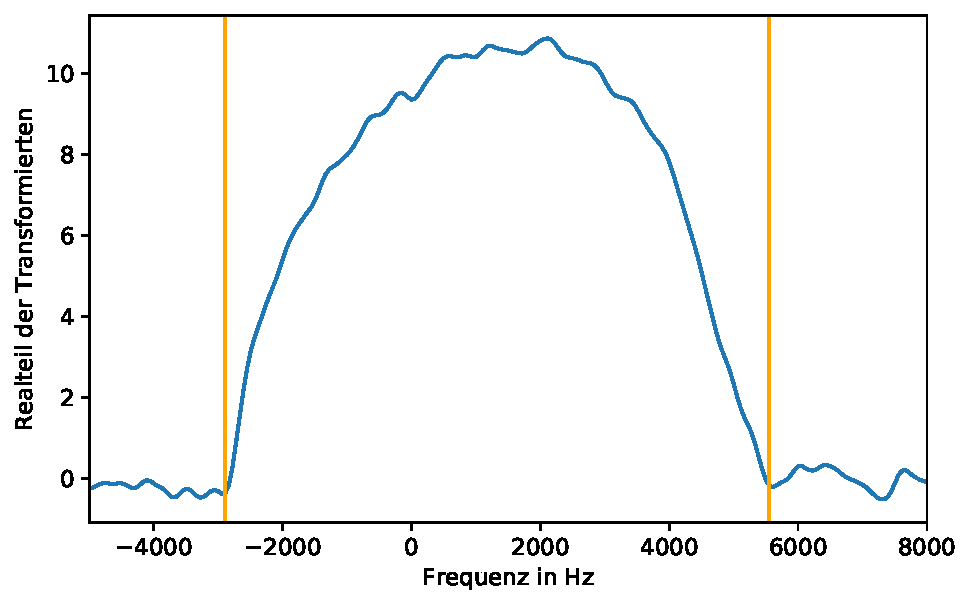
\includegraphics[scale = 0.75]{plots/fourier.pdf}
    \caption{NMR Spektrum. Fouriertransformierte des Realteils des Spin-Echos. In Orange sind die abgelesenen Ränder des Halbkreises markiert.}
    \label{fig:fourier}
\end{figure}
\subsection{Bestimmung der Diffusionskonstanten $D$ und Molekülradius $r$}
Mit dem Zusammenhang 
\begin{equation*}
    T_D = \frac{3}{D \gamma^2 G^2}
\end{equation*}
lässt sich aus der Diffusionszeit und dem Feldgradienten die Diffusionskonstante berechnen:
\begin{equation*}
    D = \sqrt{\frac{3d^2}{4\pi^2k^2T_D}} = \SI{59.58 +- 1.29 E-09}{\metre \squared  \per \second}
\end{equation*}
Mit der nun bekannten Diffusionskonstante, der gemessenen Temperatur $T = \SI{21.2}{\celsius}$ und der Viskosität von Wasser bei raumtemperatur $\eta = \SI{0.0010087}{kg\per\metre\per\second}$ lässt sich nun der Molekülradius $r$ berechnen.
\begin{equation*}
    r = \frac{k_B T}{6\pi D \eta} = \SI{358 +- 7 E-14}{\metre}
\end{equation*}
